
%
%   svt_daq.tex
%       author: Omar Moreno <omoreno1@ucsc.edu>
%               Santa Cruz Institute for Particle Physics
%               University of California, Santa Cruz
%      created: November 13, 2012
%

The expected data rates and event sizes for each of the dedicated photon runs
were estimated using a full simulation of the SVT DAQ and compared to observed
values. As discussed in Section~\ref{sec:testrun_daq}, the digitized samples
from three hybrids were received by a single DPM.  The DPM then required that
at least three of the six samples exceeded a threshold of two times the noise
level for that channel.  An additional ``pile-up'' cut requiring that 
(sample 2 $>$ sample 1) or (sample 3 $>$ sample 2) was also applied. This was
meant to eliminate hits arising from the falling edge of previous hits expected
to occur when running at the highest occupancies.
%Signals from the photon run were unaffected by such a cut. 

All samples were placed into their own container along with the 
channel number, hybrid identifier, chip address and DPM identifier. An 
additional layer of encapsulation or bank was used to store all samples 
emerging from a single DPM along with the DPM identifier, the event number
an error bit and hybrid temperatures. A diagram of the container along with
the sizes of each of the elements is shown on Figure~\ref{fig:data_format}.
\begin{figure}[h]
    \begin{center}
    	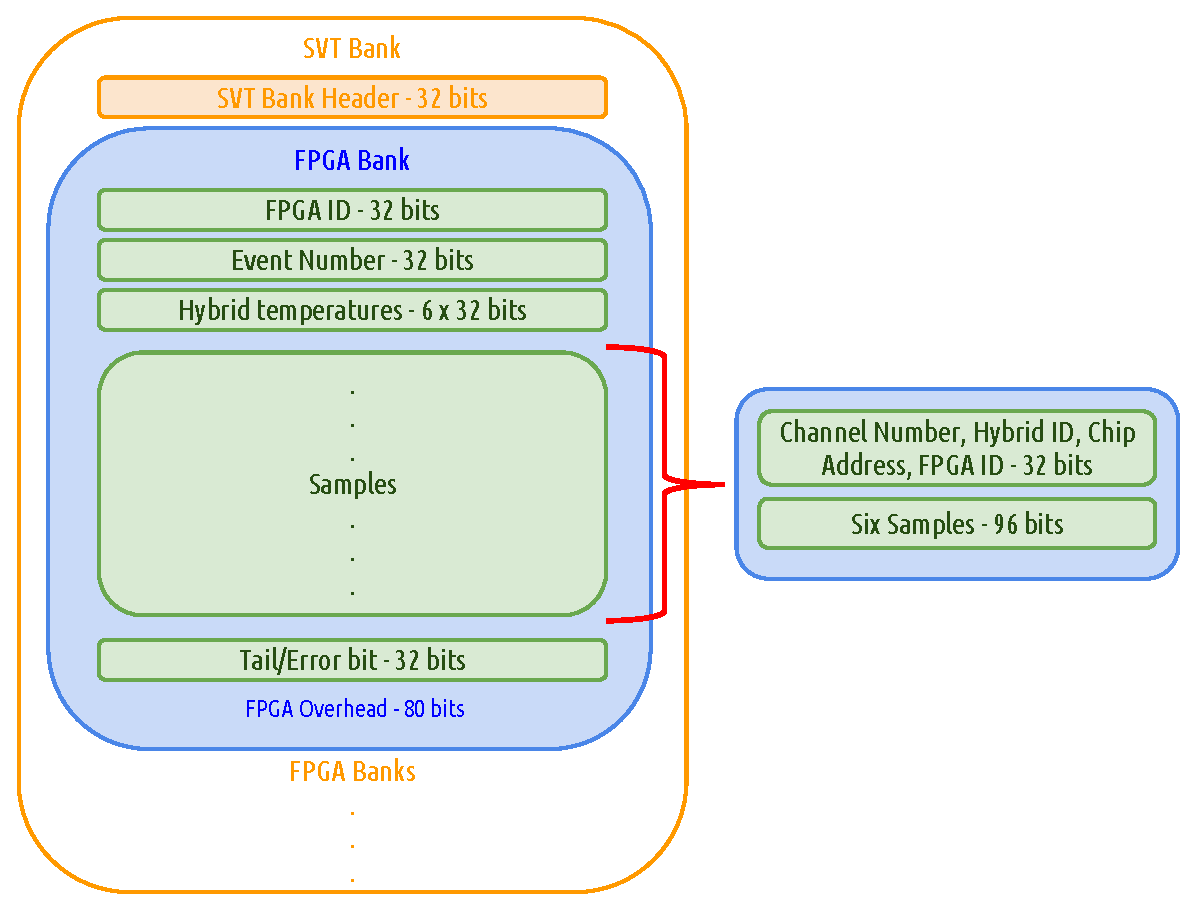
\includegraphics[width=0.60\textwidth]{test2012/svtperformance/daq/svt_data_format.pdf}
        \caption{
                    SVT data format. Samples readout from three hybrids are 
                    processed by a single FPGA and are placed within a single
                    container or FPGA bank.  An additional layer of 
                    encapsulation is used to store all of the FPGA banks.
                 } 
	\label{fig:data_format}
    \end{center}
\end{figure}
Overall, the container overhead will contribute a total of 326 bytes to an event
with an additional 16 bytes per hit.

The occupancy expected for each of the converter thicknesses along with the 
corresponding event size and data rate are shown on Table~\ref{table:sim_rates}.
\begin{table}[h]
    \scalebox{0.9}{
    \begin{tabular}{ c | c | c | c }
    \hline
    %  Are the trigger rates going to be listed anywhere else? Otherwise, they should be listed here.
    Converter Thickness (\%$X_0$) & Sim Occupancy (\%)  & Sim Event Size (kB) &   Sim Data Rate (Mb/s) \\      
    \hline 
    1.6                           & .438                & 1.22                &   2.07                 \\
    0.45                          & .293                & .93                 &   .53                  \\
    0.18                          & .118                & .56                 &   .24                  \\ 
    \end{tabular} } 
    \caption{Occupancy, event size and resulting data rate expected for each of the three 
             converter thicknesses used in the test run.}
    \label{table:sim_rates}
\end{table}
The occupancies shown include a contribution of .02\% (3 hits) due to noise and  
data rates are estimated using the trigger rates observed during each
of the dedicated photon runs. As expected i.e. thicker targets correspond to higher 
occupancies. 

Table~\ref{table:observed_rates} list the observed occupancy, event sizes and 
\begin{table}[h]
    \scalebox{0.9}{ 
        \begin{tabular}{ c | c | c | c }
            \hline
            Converter Thickness (\%$X_0$)   & Obs. Occupancy (\%) & Obs. Event Size (kB) & Obs. Data Rate (Mb/s) \\
            \hline
            1.6                             & 1.03                & 2.43                 & 4.12                  \\
            0.45                            & 1.22                & 2.82                 & 1.61                  \\
            0.18                            & 1.23                & 2.84                 & 1.21                  \\
        \end{tabular}
    }
    \caption{Occupancy, event size and resulting data rate observed for each of the three 
             converter thicknesses used in the test run.}
    \label{table:observed_rates}
\end{table}    
rates for each of the targets.  The data rates observed during the test run were
much higher than expected.  This can be attributed to a known
noisy sensor and a few noisy chips which appeared during certain runs.  The causes
of both these issues are now well understood and will be resolved for future running.

A better comparison between simulated and observed data rates can be obtained
by masking out all known noisy channels found during the commissioning of the 
SVT.  The resulting data rates are listed on Table~\ref{table:masked_rates}. 
\begin{table}[h]
    \scalebox{0.8}{ 
        \begin{tabular}{ c | c | c | c }
            \hline
            Converter Thickness (\%$X_0$)   & Obs. (Sim) Occupancy (\%) & Obs. (Sim) Event Size (kB) & Obs. (Sim) Data Rate (Mb/s) \\
            \hline
            1.6                             &  ()               &  ()                &   ()                \\
            0.45                            &  ()               &  ()                &   ()                \\
            0.18                            &  ()               &  ()                &   ()                \\
        \end{tabular}
    }
    \caption{Comparison of occupancy, event size and resulting data rate for each of the three 
             converter thicknesses used in the test run after all bad channels are masked.}
    \label{table:masked_rates}
\end{table}    
\textcolor{red}{Combine all tables into a single plot.}
